\documentclass[aspectratio=169,10pt]{beamer}
% =====================================================================
%  Presentación del artículo de la Unidad II, Finanzas I (055D), UNCP
%  Compilar con pdfLaTeX (dos veces).
% =====================================================================
\usepackage[utf8]{inputenc}
\usepackage[T1]{fontenc}
\usepackage[scaled=0.95]{helvet}
\renewcommand{\familydefault}{\sfdefault}
\usepackage{microtype}
\usepackage{amsmath}
\usepackage{graphicx}
\usepackage{booktabs}
\usepackage{tabularx}
\usepackage{array}
\usepackage{xcolor}
\usepackage{tikz}
\usetikzlibrary{positioning,arrows.meta,shapes.misc,calc}
\usepackage[most]{tcolorbox}
\usepackage{qrcode}
\usepackage{xurl}
\urlstyle{same}
\hypersetup{colorlinks=false,pdfborder={0 0 0}}

% ---------------- Paleta ----------------
\definecolor{navy}{HTML}{8E0C11}
\definecolor{navy2}{HTML}{B8121A}
\definecolor{gold}{HTML}{00A3E0}
\definecolor{acento}{HTML}{A6E1F7}
\definecolor{goldsoft}{HTML}{E8F6FC}
\definecolor{teal}{HTML}{353435}
\definecolor{rojo}{HTML}{E40001}
\definecolor{gris}{HTML}{5E5757}
\definecolor{linea}{HTML}{E5D7D7}
\definecolor{fondo}{HTML}{F6F1F1}

% ---------------- Tema propio ----------------
\setbeamertemplate{navigation symbols}{}
\setbeamercolor{normal text}{fg=black!88}
\setbeamercolor{structure}{fg=navy}
\setbeamercolor{alerted text}{fg=navy}
\setbeamerfont{frametitle}{size=\large,series=\bfseries}
\setbeamertemplate{frametitle}{%
  \nointerlineskip
  \begin{beamercolorbox}[wd=\paperwidth,ht=11mm,dp=0mm,leftskip=8mm,rightskip=8mm]{}%
    \begin{tikzpicture}[remember picture,overlay]
      \fill[navy] (current page.north west) rectangle ([yshift=-12.5mm]current page.north east);
      \fill[gold] ([yshift=-12.5mm]current page.north west) rectangle ([yshift=-13.3mm]current page.north east);
      \node[anchor=east,inner sep=0] (esc) at ([xshift=-6mm,yshift=-6.25mm]current page.north east) {\includegraphics[height=8mm]{Escudo_UNCP.png}};
      \node[anchor=east,inner sep=0] at ([xshift=-2.5mm]esc.west) {\includegraphics[height=8mm]{Logo_FE.png}};
    \end{tikzpicture}%
    \vbox to 11mm{\vfil\color{white}\usebeamerfont{frametitle}\insertframetitle\ifx\insertframesubtitle\empty\else\\[-1pt]{\footnotesize\mdseries\color{white!80}\insertframesubtitle}\fi\vfil}%
  \end{beamercolorbox}%
  \vspace{0.5mm}%
}
\setbeamertemplate{footline}{%
  \begin{tikzpicture}[remember picture,overlay]
    \fill[fondo] (current page.south west) rectangle ([yshift=6.5mm]current page.south east);
    \draw[linea] ([yshift=6.5mm]current page.south west) -- ([yshift=6.5mm]current page.south east);
    \node[anchor=west,font=\tiny,text=gris] at ([xshift=8mm,yshift=3.25mm]current page.south west) {Meglinho Sneyder Rojas Poma \,|\, Finanzas I (055D), UNCP 2026-II};
    \node[anchor=east,font=\tiny,text=gris] at ([xshift=-20mm,yshift=3.25mm]current page.south east) {Betas sectoriales y costo de capital en la BVL, 2021-2026};
    \node[anchor=east,font=\tiny\bfseries,text=navy] at ([xshift=-8mm,yshift=3.25mm]current page.south east) {\insertframenumber\,/\,\inserttotalframenumber};
  \end{tikzpicture}%
}
\setbeamertemplate{itemize items}{\textcolor{gold}{\rule[0.25ex]{0.9ex}{0.9ex}}}
\setbeamertemplate{itemize subitem}{\textcolor{navy}{\raisebox{0.2ex}{\scriptsize$\bullet$}}}
\setbeamertemplate{enumerate items}{\textcolor{navy}{\bfseries\insertenumlabel.}}
\setlength{\leftmargini}{1.3em}
\setbeamersize{text margin left=8mm,text margin right=8mm}

% ---------------- Cajas ----------------
\newtcolorbox{caja}[2][]{enhanced,sharp corners,boxrule=0pt,colback=fondo,colframe=fondo,
  left=2.6mm,right=2.6mm,top=1.6mm,bottom=1.6mm,borderline west={1.1mm}{0pt}{#2},fontupper=\footnotesize\raggedright,#1}
\newtcolorbox{clave}[1][]{enhanced,sharp corners,boxrule=0pt,colback=navy,coltext=white,
  left=2.6mm,right=2.6mm,top=1.6mm,bottom=1.6mm,fontupper=\footnotesize\raggedright\color{white},
  before upper={\setbeamercolor{itemize/enumerate body}{fg=white}\setbeamercolor{normal text}{fg=white}},#1}
\newtcolorbox{lectura}[1][]{enhanced,sharp corners,boxrule=0pt,colback=goldsoft,
  left=2.6mm,right=2.6mm,top=1.4mm,bottom=1.4mm,borderline west={1.1mm}{0pt}{gold},fontupper=\footnotesize\raggedright,#1}
\newcommand{\etiqueta}[2]{{\color{#1}\scriptsize\bfseries\MakeUppercase{#2}}\par\vspace{1mm}}
\newcommand{\fuente}[1]{\par\vspace{1mm}{\color{gris}\tiny #1\par}}
\newcommand{\num}[3]{\begin{minipage}[t]{#1}\centering{\color{navy}\Large\bfseries #2}\par\vspace{0.6mm}{\color{gris}\scriptsize #3}\end{minipage}}

\begin{document}

% =====================================================================
%  1. PORTADA
% =====================================================================
{\setbeamertemplate{footline}{}
\begin{frame}[plain]
\begin{tikzpicture}[remember picture,overlay]
  \fill[navy] (current page.north west) rectangle ([yshift=-58mm]current page.north east);
  \fill[gold] ([yshift=-58mm]current page.north west) rectangle ([yshift=-59mm]current page.north east);
  \node[anchor=north west,inner sep=0] at ([xshift=8mm,yshift=-7mm]current page.north west) {\includegraphics[height=15mm]{Escudo_UNCP.png}};
  \node[anchor=north east,inner sep=0] at ([xshift=-8mm,yshift=-7mm]current page.north east) {\includegraphics[height=15mm]{Logo_FE.png}};
  \node[anchor=north,text=acento,font=\scriptsize\bfseries] at ([yshift=-9mm]current page.north) {ARTÍCULO DE INVESTIGACIÓN \,|\, UNIDAD II \,|\, TEMA 61};
  \node[anchor=north,text=white,font=\Large\bfseries,text width=118mm,align=center] at ([yshift=-17mm]current page.north)
    {Betas sectoriales y costo de capital en un mercado ilíquido: evidencia de la Bolsa de Valores de Lima, 2021-2026};
  \node[anchor=north,text=white!78,font=\footnotesize\itshape,text width=120mm,align=center] at ([yshift=-39mm]current page.north)
    {Industry betas and the cost of capital in an illiquid market: evidence from the Lima Stock Exchange, 2021-2026};
  \node[anchor=north west,text width=100mm,font=\small] at ([xshift=8mm,yshift=-61.5mm]current page.north west) {%
    {\color{navy}\large\bfseries Meglinho Sneyder Rojas Poma}\\[1mm]
    {\color{gris}\footnotesize Código 2024200522B}\\[2mm]
    \scriptsize Escuela Profesional de Economía, Facultad de Economía\\ Universidad Nacional del Centro del Perú\\[1mm]
    Finanzas I (055D) \,|\, Docente: Dr. Ciro Iván Machacuay Meza\\ Huancayo, noviembre de 2026};
  \node[anchor=north east,inner sep=0] (qr) at ([xshift=-12mm,yshift=-62mm]current page.north east)
    {\href{https://github.com/SneyderRP/finanzas-i-tema61-costo-capital-bvl}{\qrcode[height=17mm]{https://github.com/SneyderRP/finanzas-i-tema61-costo-capital-bvl}}};
  \node[anchor=north,text=gris,font=\tiny,align=center] at ([yshift=-1.5mm]qr.south) {Datos y código\\del estudio};
\end{tikzpicture}
\end{frame}
}

% =====================================================================
%  2. CONTEXTO, PROBLEMA Y OBJETIVOS
% =====================================================================
\begin{frame}{Contexto, problema y objetivos}
\begin{columns}[T]
\begin{column}{0.5\textwidth}
\begin{caja}{navy}
\etiqueta{navy}{Por qué importa}
El costo de capital es la tasa que exigen los inversionistas; se estima con el CAPM y depende de la \textbf{beta}. Una beta mal estimada se traslada al valor de las empresas.
\end{caja}
\vspace{1mm}
\begin{caja}{rojo}
\etiqueta{rojo}{El problema en la BVL}
\begin{itemize}\setlength{\itemsep}{0.4mm}
\item Sin series históricas ni índices sectoriales oficiales.
\item Acciones que pasan semanas sin cambiar de precio \textbf{subestiman la beta} (Altay y Çalgıcı, 2019).
\item Las empresas más grandes cotizan también en Nueva York.
\end{itemize}
\end{caja}
\end{column}
\begin{column}{0.46\textwidth}
\begin{clave}
\etiqueta{acento}{Objetivo general}
Estimar la beta y el costo de capital de cuatro carteras sectoriales de la BVL entre noviembre de 2021 y octubre de 2026.\par\vspace{0.8mm}
{\color{acento}\bfseries Hipótesis:} los sectores tienen betas distintas; minería mayor que 1 y consumo menor que 1.
\end{clave}
\vspace{1mm}
\begin{caja}{gold}
\etiqueta{gold!80!black}{Objetivos específicos}
\begin{enumerate}\setlength{\itemsep}{0.4mm}
\item Construir una base propia con dos vías de extracción.
\item Estimar las betas con controles del Tesoro y del tipo de cambio.
\item Calcular el costo de capital y probar su robustez.
\end{enumerate}
\end{caja}
\end{column}
\end{columns}
\end{frame}

% =====================================================================
%  3. ANTECEDENTES
% =====================================================================
\begin{frame}{Antecedentes de la literatura}
\scriptsize
\renewcommand{\arraystretch}{1.22}
\begin{tabularx}{\textwidth}{@{}>{\raggedright\arraybackslash\bfseries\color{navy}}p{31mm} >{\raggedright\arraybackslash}X >{\raggedright\arraybackslash\color{gris}}p{38mm}@{}}
\toprule
\normalcolor\textbf{Estudio} & \textbf{Hallazgo principal} & \normalcolor\textbf{Uso en este trabajo} \\
\midrule
Hourani et al. (2023) & En 29 mercados frontera, el costo de capital por industria es impreciso porque las cargas de riesgo cambian en el tiempo. & Estimar por sector y no por país. \\
Bazhutov et al. (2023) & Las betas diarias o semanales funcionan mejor que las mensuales, y el índice elegido cambia el resultado. & Datos diarios y prueba con otro índice. \\
Altay y Çalgıcı (2019) & Agregar betas de iliquidez mejora la explicación de los retornos. & Filtro de liquidez. \\
Yildiz y Erzurumlu (2018) & En Borsa Istanbul el tipo de cambio pesa más que el índice mundial. & Tipo de cambio como control. \\
Tomtosov (2024) & Las carteras que comparten acciones generan correlación mecánica. & Mercado sin el propio sector. \\
Cepoi et al. (2025) & En empresas con doble cotización, la bolsa extranjera puede liderar la formación del precio. & Lectura de la iliquidez local. \\
Arbaa y Varon (2019) & Las crisis cambiarias se trasladan a la banca. & Exposición cambiaria. \\
\bottomrule
\end{tabularx}
\vfill
\begin{clave}
\textbf{Vacío que cubre el estudio:} la evidencia reciente para la BVL con datos diarios y por sector es escasa.
\end{clave}
\end{frame}

% =====================================================================
%  4. DATOS Y CARTERAS
% =====================================================================
\begin{frame}{Datos: dos vías de extracción y carteras sectoriales}
\centering
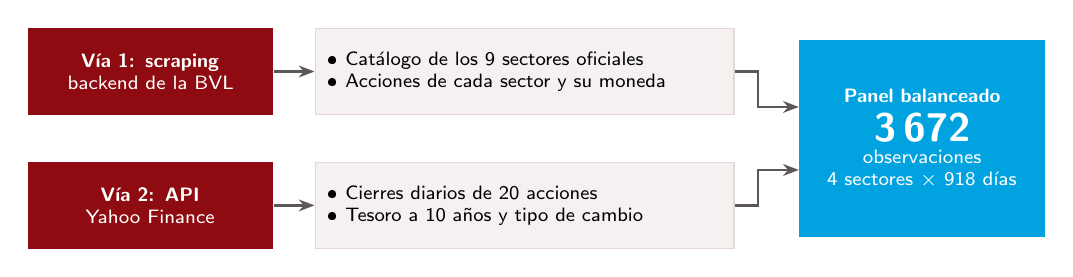
\begin{tikzpicture}[
  font=\scriptsize,
  src/.style={rectangle,fill=navy,text=white,text width=28mm,align=center,minimum height=11mm,inner sep=1.6mm},
  dst/.style={rectangle,fill=fondo,draw=linea,text width=50mm,align=left,minimum height=11mm,inner sep=1.6mm},
  fin/.style={rectangle,fill=gold,text=white,text width=28mm,align=center,minimum height=25mm,inner sep=1.6mm},
  arr/.style={-{Stealth[length=2mm]},line width=0.8pt,color=gris}]
\node[src] (bvl) at (0,0.85) {\textbf{Vía 1: scraping}\\backend de la BVL};
\node[src] (yah) at (0,-0.85) {\textbf{Vía 2: API}\\Yahoo Finance};
\node[dst] (o1) at (4.75,0.85) {\textbullet\ Catálogo de los 9 sectores oficiales\\ \textbullet\ Acciones de cada sector y su moneda};
\node[dst] (o2) at (4.75,-0.85) {\textbullet\ Cierres diarios de 20 acciones\\ \textbullet\ Tesoro a 10 años y tipo de cambio};
\node[fin] (p) at (9.8,0) {\textbf{Panel balanceado}\\[1mm]{\Large\textbf{3\,672}}\\observaciones\\4 sectores $\times$ 918 días};
\draw[arr] (bvl) -- (o1); \draw[arr] (yah) -- (o2);
\draw[arr] (o1.east) -- ++(3mm,0) |- ([yshift=4mm]p.west);
\draw[arr] (o2.east) -- ++(3mm,0) |- ([yshift=-4mm]p.west);
\end{tikzpicture}
\par\vspace{1.5mm}\raggedright
\scriptsize
\renewcommand{\arraystretch}{1.15}
\begin{tabularx}{\textwidth}{@{}>{\bfseries\color{navy}}l X c@{}}
\toprule
\normalcolor\textbf{Cartera} & \textbf{Acciones} & \textbf{N} \\
\midrule
Minería & SCCO, BVN, CVERDEC1, VOLCABC1, MINSURI1, NEXAPEC1 & 6 \\
Banca & BAP, IFS, BBVAC1 & 3 \\
Consumo & INRETC1, ALICORC1, BACKUSI1 & 3 \\
Construcción & CPACASC1, UNACEMC1, CORAREI1, SIDERC1 & 4 \\
\bottomrule
\end{tabularx}
\fuente{El mercado suma CREDITC1, FERREYC1, LUSURC1 y ENGIEC1 (20 acciones), con ponderación igual. Las acciones en dólares se convirtieron a soles con el tipo de cambio diario. El cierre de Yahoo coincidió con la BVL en 10 de 10 acciones (tolerancia de 0.5\,\%).}
\end{frame}

% =====================================================================
%  5. FILTRO DE LIQUIDEZ Y MODELO
% =====================================================================
\begin{frame}{Filtro de liquidez y modelo econométrico}
\begin{columns}[T]
\begin{column}{0.5\textwidth}
\etiqueta{navy}{Días en que el precio cambió}
\scriptsize
\renewcommand{\arraystretch}{1.1}
\begin{tabular*}{\linewidth}{@{\extracolsep{\fill}}lrr|lrr@{}}
\toprule
\multicolumn{3}{@{}l}{\textbf{Se conservan (ejemplos)}} & \multicolumn{3}{l@{}}{\textbf{Se excluyen ($<$ 30\,\%)}} \\
Acción & \% & Racha & Acción & \% & Racha \\
\midrule
SCCO & 99.7 & 2 & ATACOBC1 & 26.6 & 65 \\
BVN & 98.6 & 2 & SCOTIAC1 & 12.5 & 50 \\
VOLCABC1 & 79.6 & 6 & INTERBC1 & 11.9 & 56 \\
ALICORC1 & 74.4 & 6 & GLORIAI1 & 10.1 & 64 \\
BBVAC1 & 61.8 & 12 & CPACASI1 & 7.2 & 121 \\
NEXAPEC1 & 43.2 & 27 & \textbf{BUENAVI1} & \textbf{4.1} & \textbf{341} \\
\bottomrule
\end{tabular*}
\fuente{Racha: mayor número de días hábiles seguidos con el mismo precio. Tomado de \texttt{incidencias\_fuente.md} (Carpeta 3).}
\vspace{0.5mm}
\begin{lectura}[fontupper=\scriptsize\raggedright]
Un precio repetido genera retornos iguales a cero que sesgan la beta hacia abajo. Buenaventura cambió de precio el \textbf{4.1\,\%} de los días en Lima y el \textbf{98.3\,\%} en Nueva York.
\end{lectura}
\end{column}
\begin{column}{0.47\textwidth}
\begin{caja}{navy}
\etiqueta{navy}{Etapa 1: beta por sector (MCO)}
\vspace{-2.5mm}
\[ Y_{s,t} = \alpha_s + \beta_s X_{1,t} + c_{1,s} X_{2,t} + c_{2,s} X_{3,t} + \varepsilon_{s,t} \]
\vspace{-3mm}

{\scriptsize $X_1$: mercado; $X_2$: Tesoro a 10 años; $X_3$: tipo de cambio. Newey-West con 5 rezagos; series estacionarias (ADF, $p<.001$).}
\end{caja}
\vspace{1mm}
\begin{caja}{gold}
\etiqueta{gold!80!black}{Etapa 2: costo de capital (CAPM)}
\vspace{-2.5mm}
\[ K_{e,s} = R_f + \beta_s\,(R_m - R_f) \]
\vspace{-3mm}

{\scriptsize $R_f = 3.886\,\%$; prima realizada de 15.38\,\% ($R_m = 19.266\,\%$) y prima de referencia de 7.5\,\%.}\par\vspace{1mm}
{\scriptsize\color{teal}\textbf{Etapa 3:} frontera eficiente de Markowitz (1952), ratios de Sharpe y Treynor y alfa de Jensen.}
\end{caja}
\end{column}
\end{columns}
\end{frame}

% =====================================================================
%  6. BETAS Y CONTRASTE
% =====================================================================
\begin{frame}{Resultados: betas sectoriales y contraste $\beta_s = 1$}
\scriptsize\setlength{\tabcolsep}{3pt}
\renewcommand{\arraystretch}{1.25}
\begin{tabular*}{\textwidth}{@{\extracolsep{\fill}}lcccccccl@{}}
\toprule
\textbf{Sector} & \textbf{Beta} & \textbf{EE} & \textbf{IC 95\,\%} & $\boldsymbol{R^2}$ & $\boldsymbol{z}\,(\beta_s=1)$ & $\boldsymbol{p}$ & \textbf{Tipo de cambio} & \textbf{Decisión} \\
\midrule
\textcolor{navy}{\textbf{Minería}} & \textbf{1.616} & 0.091 & [1.438, 1.793] & .766 & 6.79 & $<.001$ & 0.019 & \textcolor{navy}{\textbf{Mayor que 1}} \\
\textcolor{navy}{\textbf{Banca}} & \textbf{1.069} & 0.093 & [0.888, 1.250] & .588 & 0.74 & .456 & $+$0.343$^{*}$ & \textcolor{gris}{Igual a 1} \\
\textcolor{navy}{\textbf{Construcción}} & \textbf{0.868} & 0.065 & [0.740, 0.996] & .399 & $-$2.02 & .043 & $-$0.290$^{*}$ & \textcolor{teal}{\textbf{Menor que 1}} \\
\textcolor{navy}{\textbf{Consumo}} & \textbf{0.547} & 0.055 & [0.440, 0.655] & .419 & $-$8.24 & $<.001$ & $+$0.209$^{*}$ & \textcolor{teal}{\textbf{Menor que 1}} \\
\bottomrule
\end{tabular*}
\fuente{$N = 918$ por sector. Errores de Newey-West con cinco rezagos. Todas las betas son significativas al 1\,\%. $^{*}$ Coeficiente del tipo de cambio significativo al 1\,\%. El Tesoro de EE.\,UU. y la constante no son significativos en ningún sector.}
\vspace{2mm}
\begin{columns}[T]
\begin{column}{0.32\textwidth}
\begin{clave}
\etiqueta{acento}{Cómo se interpreta}
Si el mercado se mueve 1\,\% en un día, la minería tiende a moverse \textbf{1.6\,\%} y el consumo solo \textbf{0.55\,\%}.
\end{clave}
\end{column}
\begin{column}{0.32\textwidth}
\begin{caja}{teal}
\etiqueta{teal}{Hipótesis}
Se confirma: los sectores tienen betas distintas. La minería amplifica el mercado, la banca se mueve con él y la construcción y el consumo lo amortiguan.
\end{caja}
\end{column}
\begin{column}{0.32\textwidth}
\begin{caja}{gold}
\etiqueta{gold!80!black}{Tipo de cambio}
Influye en tres sectores. En la banca coincide con Arbaa y Varon (2019); en la minería no es significativo.
\end{caja}
\end{column}
\end{columns}
\end{frame}

% =====================================================================
%  7. COSTO DE CAPITAL
% =====================================================================
\begin{frame}{Resultados: costo de capital por sector}
\begin{columns}[T]
\begin{column}{0.62\textwidth}
\includegraphics[width=\linewidth,height=60mm,keepaspectratio]{figuras/figura8_costo_capital.png}
\fuente{$K_e = R_f + \beta_s(R_m - R_f)$ con la prima realizada; la línea marca $R_f = 3.886\,\%$. Generada por \texttt{04\_analisis.py} (\texttt{salidas/figura8\_costo\_capital.png}).}
\end{column}
\begin{column}{0.35\textwidth}
\begin{clave}
\etiqueta{acento}{Resultado principal}
La minería exige \textbf{cerca del doble} de retorno que el consumo, con cualquiera de las dos primas: una sola tasa para toda la bolsa valoraría mal los proyectos.
\end{clave}
\vspace{1.2mm}
\begin{caja}{gold}
\etiqueta{gold!80!black}{Con dos primas}
\renewcommand{\arraystretch}{1.1}
\begin{tabular*}{\linewidth}{@{\extracolsep{\fill}}lrr@{}}
 & \textbf{15.38\,\%} & \textbf{7.5\,\%} \\
Minería & 28.73 & 16.00 \\
Banca & 20.33 & 11.90 \\
Construcción & 17.23 & 10.40 \\
Consumo & 12.31 & 7.99 \\
\end{tabular*}\par\vspace{1mm}
La prima de 7.5\,\% es más prudente que la realizada.
\end{caja}
\end{column}
\end{columns}
\end{frame}

% =====================================================================
%  8. MODELO FINANCIERO (MARKOWITZ)
% =====================================================================
\begin{frame}{Modelo financiero: frontera eficiente de Markowitz}
\begin{columns}[T]
\begin{column}{0.56\textwidth}
\includegraphics[width=\linewidth,height=58mm,keepaspectratio]{figuras/figura9_frontera_eficiente.png}
\fuente{200\,000 combinaciones de pesos no negativos (semilla 522); el color indica el ratio de Sharpe. Generada por \texttt{05\_markowitz.py} (\texttt{salidas/figura9\_frontera\_eficiente.png}).}
\end{column}
\begin{column}{0.41\textwidth}
\begin{clave}
\etiqueta{acento}{Cartera de máximo Sharpe}
Banca 40\,\%, construcción 36\,\% y minería 24\,\%: retorno de \textbf{23.1\,\%}, volatilidad de 18.3\,\% y Sharpe de \textbf{1.05}.
\end{clave}
\vspace{1mm}
\begin{caja}{gold}
\etiqueta{gold!80!black}{Mínima varianza y ganancia}
Consumo 55\,\% y construcción 37\,\%: volatilidad de \textbf{13.9\,\%}. Diversificar mejora el Sharpe en \textbf{19.1\,\%} y baja la volatilidad en \textbf{15.5\,\%}.\par\vspace{1mm}
Ningún alfa de Jensen es significativo ($p \geq .517$).
\end{caja}
\end{column}
\end{columns}
\end{frame}

% =====================================================================
%  9. ROBUSTEZ Y DIAGNÓSTICO
% =====================================================================
\begin{frame}{Robustez y diagnóstico de los residuos}
\begin{columns}[T]
\begin{column}{0.58\textwidth}
\includegraphics[width=\linewidth,height=60mm,keepaspectratio]{figuras/figura7_betas.png}
\fuente{Betas contra el mercado de 20 acciones; la línea marca la beta del mercado, igual a 1. Generada por \texttt{04\_analisis.py} (\texttt{salidas/figura7\_betas.png}).}
\end{column}
\begin{column}{0.39\textwidth}
\begin{caja}{navy}
\etiqueta{navy}{Mercado sin el propio sector}
Cada cartera forma parte del índice, lo que eleva la beta por correlación mecánica (Tomtosov, 2024). Sin el propio sector, las betas bajan a 1.093, 0.793, 0.534 y 0.379, siguen significativas al 1\,\% y el \textbf{ordenamiento no cambia}.
\end{caja}
\vspace{1mm}
\begin{caja}{teal}
\etiqueta{teal}{Diagnóstico}
Durbin-Watson entre 1.88 y 2.11: sin autocorrelación. Jarque-Bera rechaza la normalidad (curtosis de 5.9 a 17.1) por días extremos; con 918 días y Newey-West la inferencia es válida.
\end{caja}
\end{column}
\end{columns}
\end{frame}

% =====================================================================
%  10. CONCLUSIONES, LIMITACIONES Y DATOS
% =====================================================================
\begin{frame}{Conclusiones, limitaciones y datos del estudio}
\begin{columns}[T]
\begin{column}{0.44\textwidth}
\begin{enumerate}\setlength{\itemsep}{0.8mm}\scriptsize
\item Los sectores de la BVL tienen \textbf{betas distintas}: minería 1.616, banca 1.069, construcción 0.868 y consumo 0.547.
\item El costo de capital va de \textbf{12.3\,\%} a \textbf{28.7\,\%} con la prima realizada y de \textbf{8.0\,\%} a \textbf{16.0\,\%} con la de 7.5\,\%: la minería exige cerca del doble que el consumo.
\item El ordenamiento se mantiene con un mercado que excluye a cada sector.
\item El tipo de cambio influye en tres sectores; el Tesoro de EE.\,UU. no tiene efecto diario significativo.
\item Combinar los cuatro sectores eleva el Sharpe de 0.88 a 1.05; ningún alfa de Jensen es significativo.
\item En la BVL es indispensable controlar la iliquidez antes de estimar la beta.
\end{enumerate}
\end{column}
\begin{column}{0.3\textwidth}
\begin{caja}{gold}
\etiqueta{gold!80!black}{Limitaciones}
\scriptsize
\begin{itemize}\setlength{\itemsep}{0.3mm}
\item Sin prima por riesgo país.
\item Ponderación igual: sin capitalización bursátil.
\item Índice propio, no el S\&P/BVL Perú General.
\item Ventana reducida a 918 días por feriados.
\item Tipo de cambio de Yahoo con saltos de hasta 3.8\,\%.
\item Una sola beta para toda la ventana.
\end{itemize}
\end{caja}
\end{column}
\begin{column}{0.22\textwidth}
\centering
\begin{tcolorbox}[enhanced,sharp corners,boxrule=0.6pt,colframe=linea,colback=white,halign=center,left=1.5mm,right=1.5mm,top=2mm,bottom=2mm]
\href{https://github.com/SneyderRP/finanzas-i-tema61-costo-capital-bvl}{\qrcode[height=24mm]{https://github.com/SneyderRP/finanzas-i-tema61-costo-capital-bvl}}\par\vspace{1.5mm}
{\color{navy}\tiny\bfseries DATOS Y CÓDIGO}\par
{\color{gris}\tiny Base de datos, programas y bitácora del estudio}
\end{tcolorbox}
\end{column}
\end{columns}
\vfill
\begin{clave}
\centering\small\textbf{Gracias} \quad{\color{white!75}\scriptsize|\quad Meglinho Sneyder Rojas Poma \,|\, Código 2024200522B}
\end{clave}
\end{frame}

\end{document}
